% !TeX root = ../main.tex

\chapter{绪论}

\section{课题研究背景}

\subsection{加速器控制系统简介}
粒子加速器是利用电磁场不断加速真空环境下的带电粒子,使之达到很高能量的装置。粒子加速器广泛应用于基础科学、生产生活、医疗卫生、科学技术等各个领域\cite{hong2014,Clayton2015}。其中,同步辐射光源是粒子加速器在科研领域的重要应用之一。同步辐射是速度接近光速的带电粒子在电磁场的作用下发生弯转时,沿弯转轨道的切线方向发出的电磁辐射,最早是在电子同步加速器上发现的。同步辐射光源是指产生同步辐射的物理装置,它的主要设备包括注入器和电子储存环,注入器产生电子束并将其加速到所需能量,电子储存环使得电子发生弯转并产生同步辐射光。同步辐射光源具有亮度高、强波长范围宽且连续可调、方向性及偏振性好、超纯净等优异特性,广泛应用于物理、化学、材料科学、生命科学、环境科学、微电子等众多基础研究和应用研究领域。合肥光源(Hefei Light Source, HLS)由中国科学技术大学国家同步辐射实验室承建,它是我国第一台以真空紫外和软X射线为主的专用同步辐射光源,在1989年建成出光。合肥光源的主体设备是一台能量为800MeV、平均流强为360mA的电子储存环。在2009至2014年间,合肥光源进行了重大维修改造,改造后的合肥光源称为HLS-II,HLS-II的储存环束流发射度显著降低,装置稳定性改善,接近三代同步辐射光源的水平\cite{Li2016}。为了建设基于衍射极限储存环的第四代同步辐射光源,国家同步辐射实验室提出了合肥先进光源(Hefei Advanced Light Source,HALS)的构想并开展了HALS预研工程,HALS于2019年下半年开始改称为Hefei Advanced Light Facility(HALF),HALF是一个位于中低能区,覆盖中红外至软X射线波段,具有高亮度、低发射度、全空间相干的最先进的衍射极限光源\cite{Bai2016}。

加速器是复杂系统的精密集成,通常加速器会包括电子枪、微波加速、磁铁偏转与聚焦、束流测量、束流注入、束流反馈、高频加速、插入元件等多个系统,系统之间协调工作,才能保证加速器的正常工作,这是加速器控制系统首先要实现的功能。加速器运行期间,需要密切监测各个系统的工作状态,进行必要的联锁和保护,才能够保证加速器安全、稳定和高效的运行。加速器运行状态监测和联锁保护,也是加速器控制系统必需的功能。综上所述,加速器控制系统承担着加速器“大脑”的功能,直接指挥着加速器的调试、运行。一般来说,粒子加速器控制系统的具体任务如下\cite{zhao2006,Liu2006}:

\begin{enumerate}[itemindent=1em,label=(\arabic*)]
	\item 对电子枪、磁铁电源、真空、高频、微波、束调管、注入、冷却水、插入件以及束测等系统的设备进行监测和控制;
	\item 建立报警和联锁保护机制,确保操作人员和设备的安全;
	\item 提供定时及同步系统,实现相关设备间协调工作及信号同步;
	\item 建立上层物理应用软件,实现轨道校正、BBA、线性参数测量与校正、响应矩阵测量、局部凸轨、Lattice标定、束流光学参数测量及校正、插入,元件补偿、装置状态和参数分析等功能;
	\item 建立数据存档和查询系统,以网页方式提供历史数据查询与分析等功能。
\end{enumerate}

粒子加速器往往体积庞大、设备众多,其控制系统一般是基于网络的分布式控制系统,目前国内外应用最为广泛的控制系统开发工具是EPICS。EPICS是实验物理和工业控制系统(Experimental Physics and Industrial Control System)的缩写,是20世纪90年代初发展起来的大型分布式控制系统的软件运行环境和开发平台,已成功应用于全世界近百个大科学装置,涉及大型粒子加速器、高能物理探测器、大型天文望远镜等多种类型装置\cite{EPICS}。国际上,European XFEL、NSLS-II、ITER、LCLS-II、FRIB、ESS、ILC等工程项目都采用EPICS作为控制系统的软件开发平台\cite{Aghababyan2015,Carcassi2009,Wallander,Flath2017,Shen2016,Arredondo2013,carwardine-2007}。在国内,EPICS已成功应用于近年来相继完成的HLS-II、北京正负电子对撞机重大改造项目(BEPC-II)、上海同步辐射光源(SSRF)、中国散列中子源(CSNS)等大型科学工程项目中\cite{liweimin-control-2007, Zhao2007,Shen2010,C.H.Wang2011},目前正在建设中的上
海硬X射线自由电子激光装置(SHINE)和高能同步辐射光源(HEPS)等项目也采用EPICS作为控制系统的软件开发平台\cite{Lv2018a,Chu2018a}。基于EPICS的控制系统是基于网络的分布式控制系统,其架构如图~\ref{fig:epics-control-system-arch}所示,遵循所谓的“标准模型”(Standard Models),从上到下分为三层,分别为分为管理层(Supervisory controls)、前端控制层(Front End Controls)和设备控制层(Devices Controls)\cite{Kuiper1991}。

\begin{figure}[!htb]
	\centering
	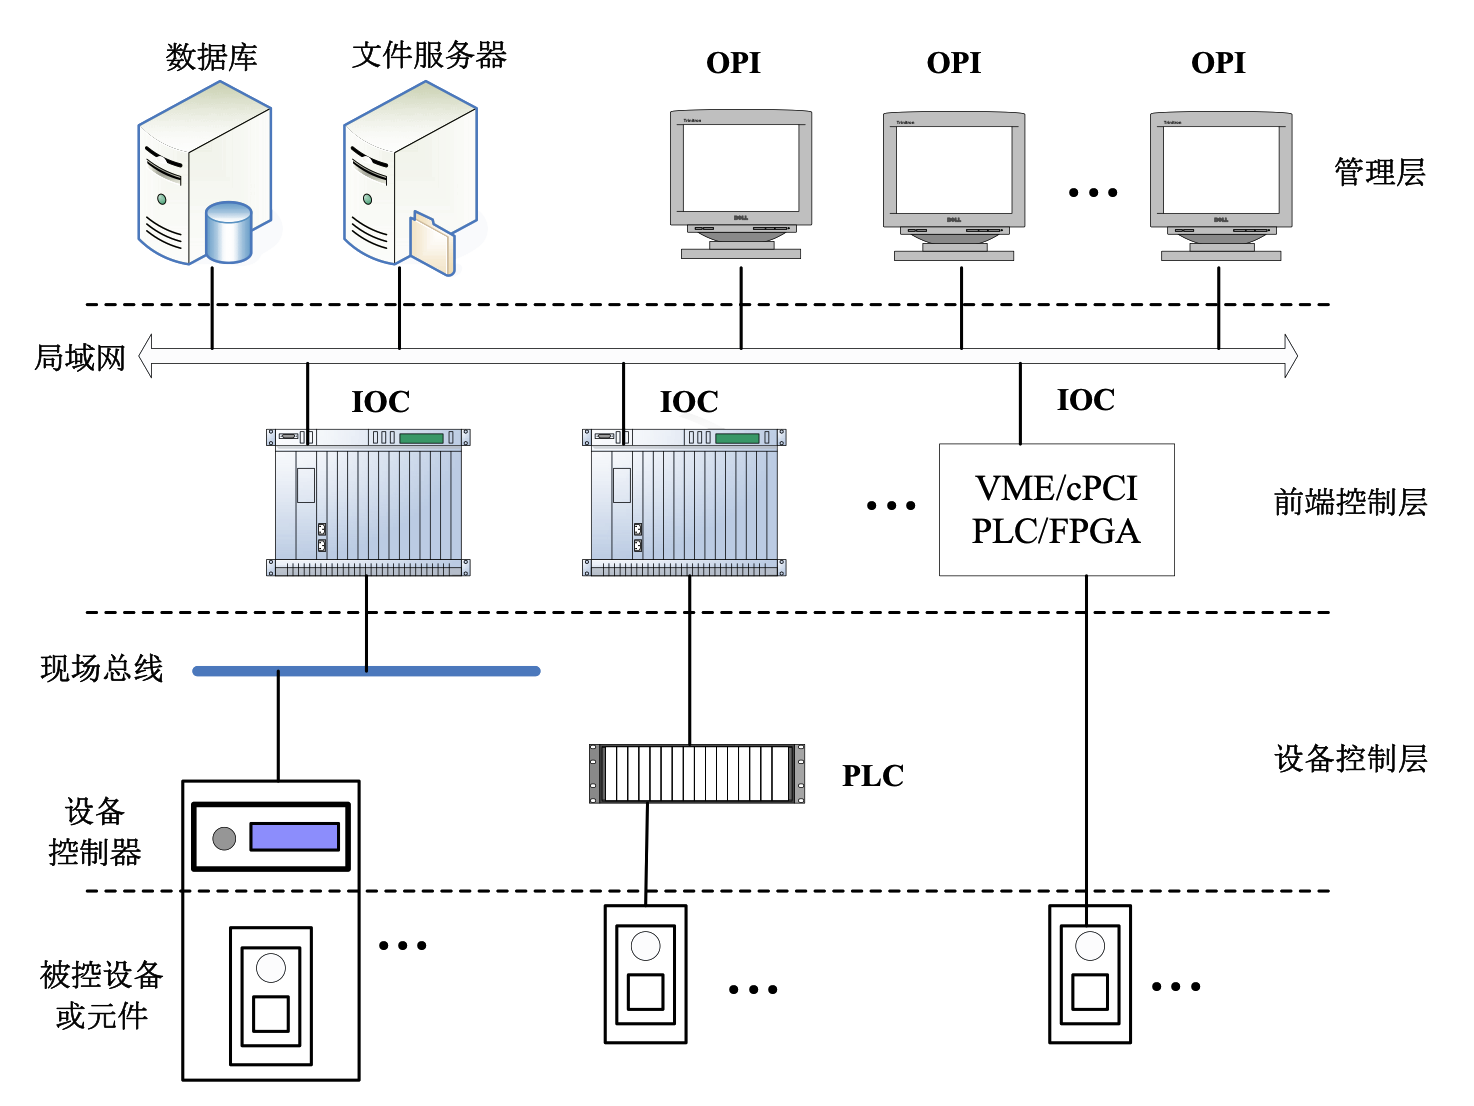
\includegraphics[width=\textwidth]{epics-control-system-arch.png}
	\caption{基于EPICS的控制系统基本结构图}
	\label{fig:epics-control-system-arch}
\end{figure}

\begin{itemize}
	\item \textbf{管理层(Supervisory controls)} \\ 
	位于系统最上层是管理层,由OPI和服务器系统组成。其中,OPI给操作人员提供了交互界面,操作人员通过OPI监控系统状态,发送控制命令。服务器系统包括数据库、文件服务器等,以提供系统初始化配置、历史数据存档和查询等功能。
	\item \textbf{前端控制层(Front End Controls)} \\ 
	前端控制层在EPICS控制系统中处于关键位置,它与管理层构成客户端/服务器(Client/Server)模式,前端控制层为服务端,管理层为客户端,二者之间通过Channel Access(CA)通信协议进行通信。前端控制器(也被称为IOC)负责输入输出控制、保存动态数据和控制算法,是控制任务的主要执行者。同时,通过CA协议将相关信息发布至管理层。
	\item \textbf{设备控制层(Devices Controls)} \\ 
	位于系统最底层的是设备控制层,是EPICS控制系统的被控对象。被控设备种类多样,有嵌入式智能设备控制器,负责控制功能复杂的设备,它们可以通过现场总线、以太网与IOC通信;也可以是PLC,用来对下层设备进行过程控制的状态监测,PLC可以通过网络或串口的方式与IOC通信。除此之外,IOC也可以通过IO模块直接对设备和元件进行控制。
\end{itemize}

\subsection{实时性分类}
实时性的含义是一个事件发生后,在确定时间内系统做出反应的能力。对于工业自动化系统来说,实时性是工业控制网络的基本要求,根据不同的应用场合,将实时性要求划分为三个范围,分别为:

\begin{enumerate}[itemindent=1em,label=(\arabic*)]
	\item 信息集成和较低要求的过程自动化应用场合,实时响应时间的要求是100ms或更长;
	\item 绝大多数的工厂自动化应用场合,实时响应时间的要求最少为5\textasciitilde10ms;
	\item 对于高性能的同步运动控制应用,特别是在100 个节点下的伺服运动控制应用场合,实时响应时间要求低于1ms,同步传送和抖动时间小于1$\mu$s\cite{liao-2005}。
\end{enumerate}

工业以太网是指用于工业自动化环境,符合IEEE 802.3标准,按照IEEE 802.1D和IEEE 802.1Q规范,并对其没有进行实时性扩展而实现的以太网。工业以太网的实时响应时间可以达到5\textasciitilde10ms,相当于现有的现场总线。对于一些实时性能要求更高的应用场合,各标准组织和公司基于工业以太网提出了各种提升实时性能的技术方案。这些方案都在IEEE 802.3标准的基础上对其进行了实时性扩展从而提高实时性能,这就是实时以太网(Real Time Ethernet,RTE)。

Ethernet POWERLINK是一种完全开源的实时以太网技术,最初由奥地利B$\&$R公司于2001年11月创立和开发,自2003年以来,由独立的用户组织EPSG负责该技术的进一步发展。POWERLINK完全建立在标准以太网(IEEE802.3)的基础之上,采用纯软件方式实现的协议,可达到硬实时的性能。EPSG在2008年发布了该技术的开源版本openPOWERLINK\cite{powerlink}。

\subsection{加速器控制系统中的实时性需求}
数据通信在粒子加速器控制系统中起着纽带的作用。随着加速器装置规模的增大和复杂度的提高,对数据通信性能的要求越来越高,而实时性是影响系统性能的关键因素,开展这方面的应用研究具有非常重要的工程应用价值。

对于加速器控制系统来说,大部分系统对实时性的要求并不高,相当于工业自动化系统的第一类场合,实时响应时间的要求是100ms 或更长,如恒温水系统的监控、真空状态的监测、慢速联锁保护等;对实时性要求较高的系统则与工业自动化系统第三类场合的要求类似,如快速联锁保护系统和电子储存环轨道快反馈系统(Fast Orbit Feedback,FOFB)等。

慢速联锁保护系统的实时响应时间要求是100ms或更长,实现方式大都采用PLC作为控制器,PLC间的通信采用标准以太网或实时以太网的软实时模式,如FERMI@Elettra FEL Facility、TPS、ESS\cite{FERMI,Liao2014,ESS}。

快速联锁保护系统的实时性要求在ms量级,一般用于束流丢失的机器保护或真空泄露的快保护等,其实现方式因应用场合的不同而有所差异。例如,上海光源的光束线前端真空泄露快保护系统采用基于FPGA和ARM的控制器,控制器间的通信参照实时以太网POWERLINK的通信方式来自主设计;西班牙ALBA的设备快速联锁系统控制器采用贝加莱公司(B$\&$R)的PLC,PLC间的通信采用实时以太网POWERLINK;美国NSLS-II的设备快速联锁系统控制器采用Allen-Bradley公司的PLC,PLC间的通信采用实时以太网Ethernet/IP;上海光源的束流丢失保护系统采用集中控制方式,将所有140个BPM信号汇总到NI PXI的FPGA板卡中,以提高系统的实时性;西班牙ALBA的束流丢失保护系统采用了专门设计的技术,将MRF定时技术的单向数据传输改进为双向数据传输,以实现高的实时性。

电子储存环轨道快反馈频率达KHz量级,反馈周期为ms量级,不同的装置所采用的方法差异较大。例如,上海光源轨道快反馈系统采用反射内存方式在10个站点间共享数据,每个站点采用2台VME计算机,分别用作轨道数据的采集和反馈校正\cite{liu-2010};英国Diamond轨道快反馈系统采用RocketIO来构建数据传输网络,通信速度是2.12Gbps\cite{DIAMOND-FOFB};美国NSLS-II轨道快反馈系统采用自主研发的串行通信接口SDI在30个计算节点间传输数据,系统快反馈频率可以达到10KHz\cite{NSLS-II-FOFB}。

从上述的解决加速器装置控制中高实时性问题的技术路线来看,有的采用自主设计的专用通信方案,有的采用实时以太网等通用技术。一般来说,通用技术较专用技术具有更好的开放性和灵活性,并可以节省产品的开发成本,缩短开发周期。因此,应该在粒子加速器控制领域中加强对实时以太网技术的研究和应用。

Ethernet POWERLINK作为一种开源的实时以太网技术,其开源性对加速器装置控制系统来说具有特别重要的意义。在加速器装置控制技术的发展过程中,开放和共享一直是其发展的方向,现在流行的控制系统开发平台无一例外都是开源的,如EPICS、TANGO、DOOCS等。

\section{国内外研究现状}
POWERLINLK已在工业控制领域得到了广泛的研究和应用\cite{xu-2015,zhu-2014,shi-2012,huang-2012,Seno-2007,cena-2009},目前在加速器控制领域,与POWERLINK相关的研究和应用还很少。国际上只有西班牙ALBA将POWERLINK用于设备保护系统,国内只有上海光源在开发光束线前端真空泄露快保护系统时,控制器间的通信设计参考了POWERLINK的通信方式。而在应用最广泛的EPICS系统中,目前还未见与POWERLINK相关的文献。

\subsection{基于POWERLINK的ALBA设备保护系统}
ALBA是一台三代同步辐射光源,建造于西班牙的巴塞罗那,于2012年建成投入使用。ALBA由直线加速器、满能量增强器和储存环组成,其中电子储存环的能量为3GeV,周长为270米,直线加速器产生并加速电子束流至100MeV,低发射度的增强器加速电子束流至满能量3Gev。ALBA目前拥有八条光束线,包括软X射线和硬X射线,主要用于生物科学、凝聚态物质、纳米科学和材料科学的研究。ALBA的设备保护系统(Equipment Protection System,EPS)的任务是避免装置组件受到损害。EPS保护范围广,不仅涵盖了ALBA加速器及其光束线,还有例如射频,光学,真空等实验室。除此之外,EPS还备份了快速联锁系统的所有信号。目前,EPS共管理数千个联锁信号,其中对数百个联锁信号需要提供毫秒量级的保护动作。

ALBA的EPS采用B$\&$R公司的X20CP1484型号PLC作为控制器,采用分布式I/O模块作为现场设备,其硬件架构如图~\ref{fig:alba-eps-arch}所示。负责加速器设备保护的PLC共有56台,PLC之间的通信周期要求达到20ms以下,采用百兆以太网POWERLINK技术实现。分布式I/O模块安装在加速器隧道内的铅屏蔽箱中,共有110个I/O模块通过X2X总线与PLC通信\cite{Alba-eps}。PLC通过以太网接入基于Tango的ALBA主控制系统局域网中,一台Tango的设备服务器通过基于以太网TCP/IP的Mobus协议来轮询PLC,从而监控EPS的状态。

\begin{figure}[!htb]
	\centering
	
\includegraphics[width=\textwidth]{alba-eps-arch.png}
	\caption{ALBA设备联锁保护系统架构图}
	\label{fig:alba-eps-arch}
\end{figure}

EPS主要包括六个子系统,分别是:真空,磁铁,射频,插入件、前端设备和光束线。每条光束线都有一个独立的EPS系统,并全部接入到加速器的EPS中。每个子系统除了本地保护逻辑之外,当子系统中某些设备状态异常时时,EPS应立即通知其他相关子系统做出保护动作。例如,当真空阀由于真空管道中的压力超过阈值而关闭,EPS应立即关闭高频系统并切断束流。每个子系统由相关PLC负责,子系统之间的联锁信号都是通过POWERLINK来进行传输。


\subsection{CERN在辐射区域关于POWERLINK的应用研究}
欧洲核子中心(Conseil Européenn pour la Recherche Nucléaire,CERN)位于瑞士日内瓦,是世界上最大的粒子物理实验室,建设了包括周长26.7千米的大型强子对撞机(Large Hadron Collider,LHC)、周长6.9千米的超级质子同步加速器(Super Proton Synchrotron,SPS)等多个加速器和一个反质子减速器 (Antiproton Decelerator,AD)。

CERN加速器装置控制系统的硬件架构可以分成三层,分别是前端层、现场总线层和分布式I/O层,如图~\ref{fig:cern-hardware-arch}所示。其中,前端层是PLC、VME、PICMG 1.3、MTCA.4等总线控制器,控制器通过现场总线和工业以太网来对分布式I/O层的不同设备进行控制。CERN现场总线层的通讯需求如表\ref{table:1.1}所示,CERN在不同区域内采用了不同的通信技术,在无辐射区域采用Profibus总线和Profinet工业以太网技术,对靠近LHC装置的辐射区域则采用耐辐射的WorldFIP总线技术\cite{Daniluk2017}。

\begin{figure}[!htb]
	\centering
	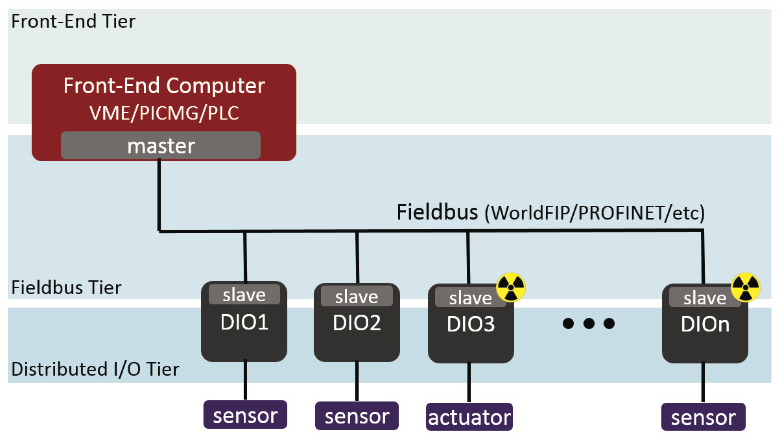
\includegraphics[width=\textwidth]{cern-hardware-arch.png}
	\caption{CERN的硬件架构图}
	\label{fig:cern-hardware-arch}
\end{figure}

\begin{table}[hbt]
  \centering
  \caption{CERN现场总线层的通讯需求}
  \label{table:1.1}
  \setlength{\tabcolsep}{15mm}
  \begin{tabular}{cc}
    \toprule

    characteristic & value\\
    \midrule
    topology & mainly daisy chain\\
    
    nodes & 100\\
    
    cycle time & 1ms\\
    
    synchronization  & 100μs\\
    
    data-per-cycle & 1Kbyte\\              
    \bottomrule
  \end{tabular}

\end{table}

在CERN的最新研究计划中,在现场总线层加入了POWERLINK实时以太网技术。POWERLINK作为唯一开源的可支持多种平台实时以太网技术,完全满足表\ref{table:1.1}所示的通讯需求。目前,CERN已在现有芯片如NetX52上实现了Profinet、POWERLINK等四种实时以太网协议,但是现有芯片不能工作在辐射区域内。CERN计划在辐射区域内采用Microsemi公司的耐辐射FPGA芯片来实现POWERLINK协议,直接可以与无辐射区域的支持POWERLINK的现有芯片直接通信。这种升级不需要替换所有已安装的设备,极大节省了人力物力。

\subsection{上海光源的光束线前端真空泄漏快保护系统}
上海光源是我国建造的第一台三代中能同步辐射光源,由一台150MeV的直线加速器,输运线,将电子束加速到到3.5GeV的满能量增强器,周长432米的3.5GeV电子储存环、八条光束线和数个实验站组成。其中光束线由安装在真空室中的一系列光学元件组成,在加速器正常运行期间,光束线的真空室是对储存环开放的。当光束线发生真空快泄漏事故的时,为防止真空泄漏扩散,真空保护快阀必须立即关闭。由于同步辐射光的直接照射会打坏真空保护快阀,因此必须在真空快阀关闭前,切断储存环的束流。位于光束线接口处的真空泄漏快保护系统作为整个光源机器保护系统的一部分,需要在真空泄漏信号给出后1ms内切断储存环束流。

上海光源的光束线前端真空泄漏快保护系统的IO站点数为20,时间响应需求是在1ms内,完成所有IO站点的之间的实时数据传输\cite{liu-2010}。系统内各节点的硬件平台是FPGA和实时以太网,通讯协议的设计参考了实时以太网POWERLINK的PRC(PollResponse Chaining)通讯模式,按照时间分片的原理来传输实时数据,各从站在各自的时间片内传输实时数据,避免两个或者多个从站同时发送数据,从而避免数据冲突,通信机制如图~\ref{fig:time-slice-principle}所示。

\begin{figure}[!htb]
	\centering
	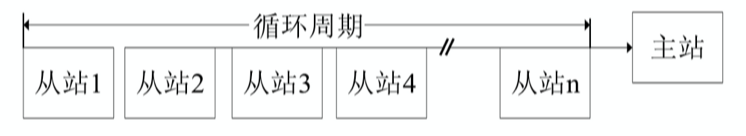
\includegraphics[width=0.75\textwidth]{time-slice-principle.png}
	\caption{时间分片原理图}
	\label{fig:time-slice-principle}
\end{figure}

第一阶段,主站的时钟与所有从站时钟同步。第二阶段,在传输数据的第一个循环周期内,先进行主时钟与第一个节点时钟的同步,再按照时间分片原理进行数据传输;在第二个循环周期内,先进行主时钟与第二个节点时钟的同步,再按照时间分片原理进行数据传输;在n+1个循环周期内,先进行主时钟与第一个节点时钟的同步,再按照时间分片原理进行数据传输,依次类推。


\section{论文工作的主要内容及创新点}

本论文的主要研究内容为实时以太网POWERLINK在粒子加速器控制系统中的应用研究。首先,我们将对加速器控制系统中实时性需求进行详细分析,并调研POWERLINK在国内外加速器控制系统中的应用,然后开展对POWERLINK通信协议的研究,解析POWERLINK协议并进行POWERLINK性能测试;其次在EPICS环境下设计基于POWERLINK设计分布式IO控制系统,设计并开发基于Zynq的前端控制器以及EPICS设备驱动程序;然后我们将搭建原型系统并进行相关实时性能测试,并且采用理论计算和仿真建模分析两种方法来对多节点的分布式控制系统解决方案的通信周期进行对比研究,确定方案可行性;最后,我们基于POWERLINK和FPGA控制器设计HALF设备保护系统,并搭建相关原型系统验证了技术方案的可行性。

本文分为五个章节,每章节的主要内容的简介如下:

第一章为绪论。本章介绍了课题研究背景,包括加速器控制系统简介、实时性分类以及加速器控制系统中的实时性分类。然后进行了国内外研究现状调研,包括基于POWERLINK的ALBA设备保护系统、CERN在辐射区域关于POWERLINK的应用研究和上海光源的光束线前端真空泄漏快保护系统。最后阐明了本课题的研究意义。

第二章为POWERLINK通信协议研究。本章首先介绍了实时以太网的概念,并对比了5种主流实时以太网的性能。随后详细介绍了POWERLINK实时以太网技术,包括POWERLINK协议的通信机制、网络模型和数据帧结构。然后介绍了POWERLINK的实现方式,包括基于Linux实现POWERLINK协议和基于FPGA实现POWERLINK协议。最后提出了理论分析和仿真建模两种方法对POWERLINK通信周期进行分析和评估。

第三章为EPICS环境下基于POWERLINK的分布式IO系统。本章提出了两套基于POWERLINK的EPICS分布式IO控制系统方案,其中第二套方案是第一套方案的升级版本。本章分别介绍了两套方案的系统架构设计、软硬件设计与开发,并分别搭建了相应的系统进行了相关性能测试。然后,基于系统的具体测试情况,我们进一步完善了理论计算方法,并验证了仿真建模方法的可行性。

第四章为HLAF设备联锁系统的设计。本章首先介绍了课题研究背景,并对国内外设备保护系统进行了调研,基于千兆POWERLINK技术和Zynq控制器设计了HALF设备保护系统。随后阐述了HLAF设备联锁保护系统的联锁保护逻辑。然后通过理论计算和网络模拟两种方法评估了设计方案的实时性能。最后我们设计了HALF EPS报警系统和HALF EPS的历史数据存档与查询系统。

第五章为论文的工作总结与展望。


本文的主要创新点为:
\begin{enumerate}
	\item 通过自主开发的驱动程序,首次将POWERLINK集成EPICS架构中,拓展了EPICS的应用范围。
	\item 基于千兆POWERLINK技术和Zynq控制器设计了HALF设备保护系统,并通过理论计算和网络模拟两种方法评估了方案的实时性能。
\end{enumerate}

